%
% einleitung.tex -- Beispiel-File für die Einleitung
%
% (c) 2020 Prof Dr Andreas Müller, Hochschule Rapperswil
%
% !TEX root = ../../buch.tex
% !TEX encoding = UTF-8
%

\section{Grundlagen der Fourier-Analyse\label{fourier:section:teil0}}
\kopfrechts{Teil 0}

Die Fourier-Analyse ist ein sehr mächtiges Mittel in der Signal-Analyse. 
Einleitung...


\subsection{Fourierreihe\label{fourier:subsection:fourierreihe}}

Mit der Fourier-Reihe lassen sich periodisch wiederholende Funktionen, wie ein Rechteck- oder Dreiecksignal, mit skalierten Sinus- und Kosinus-Schwingungen darstellen.
Um die Reihe aufzustellen, braucht man nur 3 Koeffizienten zu bestimmen. 

\begin{itemize}
	\item $a_0$ ist der Mittelwert, der Funktion. 
	Dieser entspricht dem Integral über eine Periode und schliesslich geteilt durch die Periode. 
	
	\begin{equation}
		a_0 = \frac{1}{T} \int_{t_0}^{t_0 + T} f(t) \, dx
	\end{equation}
	
	\item $a_n$ beschreibt den geraden Anteil der Funktion.
	
	\begin{equation}
		a_n = \frac{2}{T} \int_{t_0}^{t_0 + T} f(t) \cos\left(\frac{2\pi n t}{T}\right) dt
	\end{equation}
	
	\item $b_n$ beschreibt den ungeraden Anteil der Funktion.
	
	\begin{equation}
		b_n = \frac{2}{T} \int_{t_0}^{t_0 + T} f(t) \sin\left(\frac{2\pi n t}{T}\right) dt
	\end{equation}
	
\end{itemize}

Mit allen Koeffizienten bestimmt lässt sich die ursprüngliche Funktion nachahmen.
Bei Funktionen mit Sprungstellen tritt das Gibbsche Phänomen auf.
Dies erklärt einen Überschwinger nach einem Sprung. Auch wenn man die unendliche Summe bildet, wird dieser Überschwinger nicht verschwinden.
Das $=$ Zeichen stimmt also nur bedingt.
Anhand der Abbildung ... sieht man sehr schön, wie die Rechteckfunktion mit Schwingungen nachgeahmt wird.

\[
f(t) = \frac{a_0}{2} + \sum_{n=1}^{\infty} \left( a_n \cos\left( \frac{2\pi n}{T} x \right) + b_n \sin\left( \frac{2\pi n}{T} x \right) \right)
\]

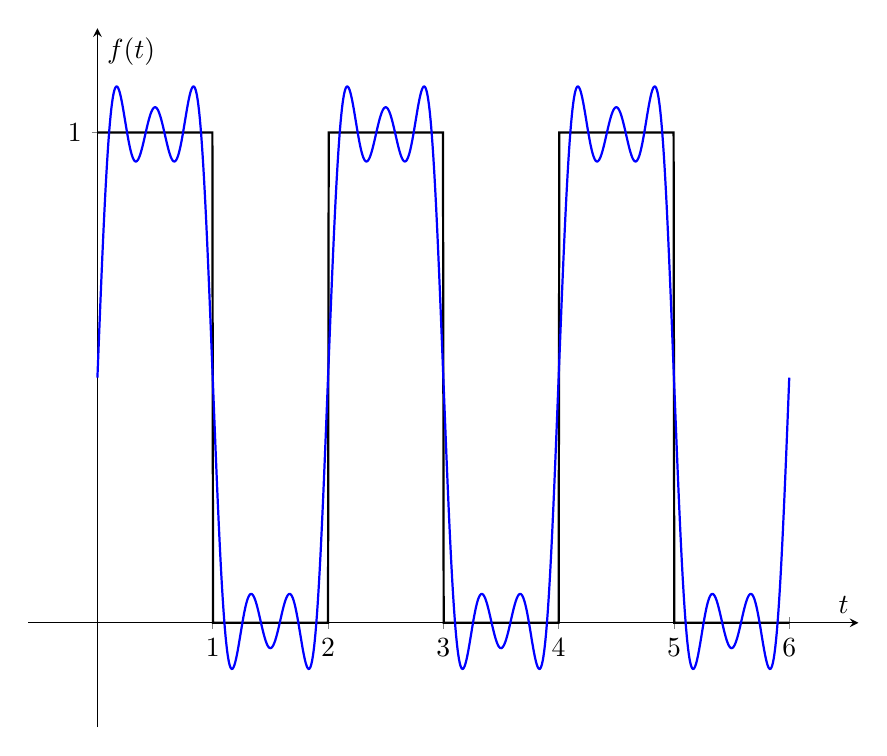
\begin{tikzpicture}
	\begin{axis}[
		axis lines = middle,
		xlabel = {$t$},
		ylabel = {$f(t)$},		
		domain=0:6,
		samples=1000,
		xtick={0,1,2,3,4,5,6},
		ytick={0,1},
		enlargelimits,
		width=\textwidth
		]
		\addplot[thick] {mod(floor(x),2) == 0 ? 1 : 0};
		\addplot[blue, thick] {(1/2) + 
			(2/pi)*sin(pi * deg(x)) + 
			(2/(3*pi))*sin(pi *3*deg(x)) +
			(2/(5*pi))*sin(pi *5*deg(x))};
	\end{axis}
\end{tikzpicture}

$a_0$ ist bei 


\subsection{Fouriertransformation\label{fourier:subsection:fouriertransformation}}

